\documentclass[twoside]{book}

% Packages required by doxygen
\usepackage{calc}
\usepackage{doxygen}
\usepackage{graphicx}
\usepackage[utf8]{inputenc}
\usepackage{makeidx}
\usepackage{multicol}
\usepackage{multirow}
\usepackage{textcomp}
\usepackage[table]{xcolor}

% Font selection
\usepackage[T1]{fontenc}
\usepackage{mathptmx}
\usepackage[scaled=.90]{helvet}
\usepackage{courier}
\usepackage{amssymb}
\usepackage{sectsty}
\renewcommand{\familydefault}{\sfdefault}
\allsectionsfont{%
  \fontseries{bc}\selectfont%
  \color{darkgray}%
}
\renewcommand{\DoxyLabelFont}{%
  \fontseries{bc}\selectfont%
  \color{darkgray}%
}

% Page & text layout
\usepackage{geometry}
\geometry{%
  a4paper,%
  top=2.5cm,%
  bottom=2.5cm,%
  left=2.5cm,%
  right=2.5cm%
}
\tolerance=750
\hfuzz=15pt
\hbadness=750
\setlength{\emergencystretch}{15pt}
\setlength{\parindent}{0cm}
\setlength{\parskip}{0.2cm}
\makeatletter
\renewcommand{\paragraph}{%
  \@startsection{paragraph}{4}{0ex}{-1.0ex}{1.0ex}{%
    \normalfont\normalsize\bfseries\SS@parafont%
  }%
}
\renewcommand{\subparagraph}{%
  \@startsection{subparagraph}{5}{0ex}{-1.0ex}{1.0ex}{%
    \normalfont\normalsize\bfseries\SS@subparafont%
  }%
}
\makeatother

% Headers & footers
\usepackage{fancyhdr}
\pagestyle{fancyplain}
\fancyhead[LE]{\fancyplain{}{\bfseries\thepage}}
\fancyhead[CE]{\fancyplain{}{}}
\fancyhead[RE]{\fancyplain{}{\bfseries\leftmark}}
\fancyhead[LO]{\fancyplain{}{\bfseries\rightmark}}
\fancyhead[CO]{\fancyplain{}{}}
\fancyhead[RO]{\fancyplain{}{\bfseries\thepage}}
\fancyfoot[LE]{\fancyplain{}{}}
\fancyfoot[CE]{\fancyplain{}{}}
\fancyfoot[RE]{\fancyplain{}{\bfseries\scriptsize Generated on Tue Mar 14 2017 12\-:38\-:12 for M\-E\-T\-I\-S by Doxygen }}
\fancyfoot[LO]{\fancyplain{}{\bfseries\scriptsize Generated on Tue Mar 14 2017 12\-:38\-:12 for M\-E\-T\-I\-S by Doxygen }}
\fancyfoot[CO]{\fancyplain{}{}}
\fancyfoot[RO]{\fancyplain{}{}}
\renewcommand{\footrulewidth}{0.4pt}
\renewcommand{\chaptermark}[1]{%
  \markboth{#1}{}%
}
\renewcommand{\sectionmark}[1]{%
  \markright{\thesection\ #1}%
}

% Indices & bibliography
\usepackage{natbib}
\usepackage[titles]{tocloft}
\setcounter{tocdepth}{3}
\setcounter{secnumdepth}{5}
\makeindex

% Hyperlinks (required, but should be loaded last)
\usepackage{ifpdf}
\ifpdf
  \usepackage[pdftex,pagebackref=true]{hyperref}
\else
  \usepackage[ps2pdf,pagebackref=true]{hyperref}
\fi
\hypersetup{%
  colorlinks=true,%
  linkcolor=blue,%
  citecolor=blue,%
  unicode%
}

% Custom commands
\newcommand{\clearemptydoublepage}{%
  \newpage{\pagestyle{empty}\cleardoublepage}%
}


%===== C O N T E N T S =====

\begin{document}

% Titlepage & ToC
\hypersetup{pageanchor=false}
\pagenumbering{roman}
\begin{titlepage}
\vspace*{7cm}
\begin{center}%
{\Large M\-E\-T\-I\-S \\[1ex]\large 1 }\\
\vspace*{1cm}
{\large Generated by Doxygen 1.8.6}\\
\vspace*{0.5cm}
{\small Tue Mar 14 2017 12:38:12}\\
\end{center}
\end{titlepage}
\clearemptydoublepage
\tableofcontents
\clearemptydoublepage
\pagenumbering{arabic}
\hypersetup{pageanchor=true}

%--- Begin generated contents ---
\chapter{Main Page}
\label{index}\hypertarget{index}{}\#\-Midterm-\/\-Metis \href{https://travis-ci.org/ltsimps/Midterm}{\tt !\mbox{[}Build Status\mbox{]}(https\-://travis-\/ci.\-org/ltsimps/\-Midterm.\-svg?branch=master)}

\subsection*{\href{https://coveralls.io/github/ltsimps/Midterm?branch=master}{\tt !\mbox{[}Coverage Status\mbox{]}(https\-://coveralls.\-io/repos/github/ltsimps/\-Midterm/badge.\-svg?branch=master)} }

\subsection*{Overview}

Initial Midterm Commit
\begin{DoxyItemize}
\item cmake
\item googletest
\end{DoxyItemize}

\#\-Description of Project

\subsection*{S\-I\-P Documentation}


\begin{DoxyItemize}
\item Product Backlog \href{https://docs.google.com/spreadsheets/d/1k9nfP__eNjIogFFWyNJw3ogN-HQ8udzpHaOekOiXbZU/edit?usp=sharing}{\tt https\-://docs.\-google.\-com/spreadsheets/d/1k9nf\-P\-\_\-\-\_\-e\-Nj\-Iog\-F\-F\-Wy\-N\-Jw3og\-N-\/\-H\-Q8udzp\-Ha\-Oek\-Oi\-Xb\-Z\-U/edit?usp=sharing}
\item Iteratartion Backlog \href{https://docs.google.com/a/terpmail.umd.edu/spreadsheets/d/1wB8Fqtjaw88LNrhkzxSVgAWAnU5Pb_bEJZ7RIEKxKpw/edit?usp=sharing}{\tt https\-://docs.\-google.\-com/a/terpmail.\-umd.\-edu/spreadsheets/d/1w\-B8\-Fqtjaw88\-L\-Nrhkzx\-S\-Vg\-A\-W\-An\-U5\-Pb\-\_\-b\-E\-J\-Z7\-R\-I\-E\-Kx\-Kpw/edit?usp=sharing}
\end{DoxyItemize}

\subsection*{Installation}


\begin{DoxyItemize}
\item Checkout the repo (and submodules) ``` \$ git clone --\href{https://github.com/ltsimps/Midterm.git}{\tt https\-://github.\-com/ltsimps/\-Midterm.\-git}
\end{DoxyItemize}

```

\subsection*{References}

Minqing Hu and Bing Liu. \char`\"{}\-Mining and Summarizing Customer Reviews.\char`\"{} Proceedings of the A\-C\-M S\-I\-G\-K\-D\-D International Conference on Knowledge Discovery and Data Mining (K\-D\-D-\/2004), Aug 22-\/25, 2004, Seattle, Washington, U\-S\-A, Bing Liu, Minqing Hu and Junsheng Cheng. \char`\"{}\-Opinion Observer\-: Analyzing 
        and Comparing Opinions on the Web.\char`\"{} Proceedings of the 14th International World Wide Web conference (W\-W\-W-\/2005), May 10-\/14, 2005, Chiba, Japan.

Theresa Wilson, Janyce Wiebe, Paul Hoffmann Recognizing Contextual Polarity in Phrase-\/\-Level \hyperlink{classSentiment}{Sentiment} Analysis Intelligent Systems Program Department of Computer Science Intelligent Systems Program University of Pittsburgh University of Pittsburgh University of Pittsburgh Pittsburgh, P\-A 15260 Pittsburgh, P\-A 15260 Pittsburgh, P\-A 15260 \href{mailto:twilson@cs.pitt.edu}{\tt twilson@cs.\-pitt.\-edu} \href{mailto:wiebe@cs.pitt.edu}{\tt wiebe@cs.\-pitt.\-edu} \href{mailto:hoffmanp@cs.pitt.edu}{\tt hoffmanp@cs.\-pitt.\-edu} \href{http://people.cs.pitt.edu/~wiebe/pubs/papers/emnlp05polarity.pdf}{\tt http\-://people.\-cs.\-pitt.\-edu/$\sim$wiebe/pubs/papers/emnlp05polarity.\-pdf} 
\chapter{Hierarchical Index}
\section{Class Hierarchy}
This inheritance list is sorted roughly, but not completely, alphabetically\-:\begin{DoxyCompactList}
\item \contentsline{section}{Parser}{\pageref{classParser}}{}
\item \contentsline{section}{Sentiment}{\pageref{classSentiment}}{}
\begin{DoxyCompactList}
\item \contentsline{section}{Negative\-Sentiment}{\pageref{classNegativeSentiment}}{}
\item \contentsline{section}{Positive\-Sentiment}{\pageref{classPositiveSentiment}}{}
\end{DoxyCompactList}
\end{DoxyCompactList}

\chapter{Class Index}
\section{Class List}
Here are the classes, structs, unions and interfaces with brief descriptions\-:\begin{DoxyCompactList}
\item\contentsline{section}{\hyperlink{classNegativeSentiment}{Negative\-Sentiment} }{\pageref{classNegativeSentiment}}{}
\item\contentsline{section}{\hyperlink{classParser}{Parser} }{\pageref{classParser}}{}
\item\contentsline{section}{\hyperlink{classPositiveSentiment}{Positive\-Sentiment} }{\pageref{classPositiveSentiment}}{}
\item\contentsline{section}{\hyperlink{classSentiment}{Sentiment} }{\pageref{classSentiment}}{}
\end{DoxyCompactList}

\chapter{File Index}
\section{File List}
Here is a list of all documented files with brief descriptions\-:\begin{DoxyCompactList}
\item\contentsline{section}{app/\hyperlink{Parser_8cpp}{Parser.\-cpp} \\*Class that handles all input and parses it out into a format that Semantics class can use }{\pageref{Parser_8cpp}}{}
\item\contentsline{section}{include/{\bfseries lib.\-hpp} }{\pageref{lib_8hpp}}{}
\item\contentsline{section}{include/{\bfseries Negative\-Sentiment.\-hpp} }{\pageref{NegativeSentiment_8hpp}}{}
\item\contentsline{section}{include/\hyperlink{Parser_8hpp}{Parser.\-hpp} \\*\hyperlink{classParser}{Parser} Class Definition. Class designed to process user input }{\pageref{Parser_8hpp}}{}
\item\contentsline{section}{include/{\bfseries Positive\-Sentiment.\-hpp} }{\pageref{PositiveSentiment_8hpp}}{}
\item\contentsline{section}{include/{\bfseries Sentiment.\-hpp} }{\pageref{Sentiment_8hpp}}{}
\end{DoxyCompactList}

\chapter{Class Documentation}
\hypertarget{classNegativeSentiment}{\section{Negative\-Sentiment Class Reference}
\label{classNegativeSentiment}\index{Negative\-Sentiment@{Negative\-Sentiment}}
}
Inheritance diagram for Negative\-Sentiment\-:\begin{figure}[H]
\begin{center}
\leavevmode
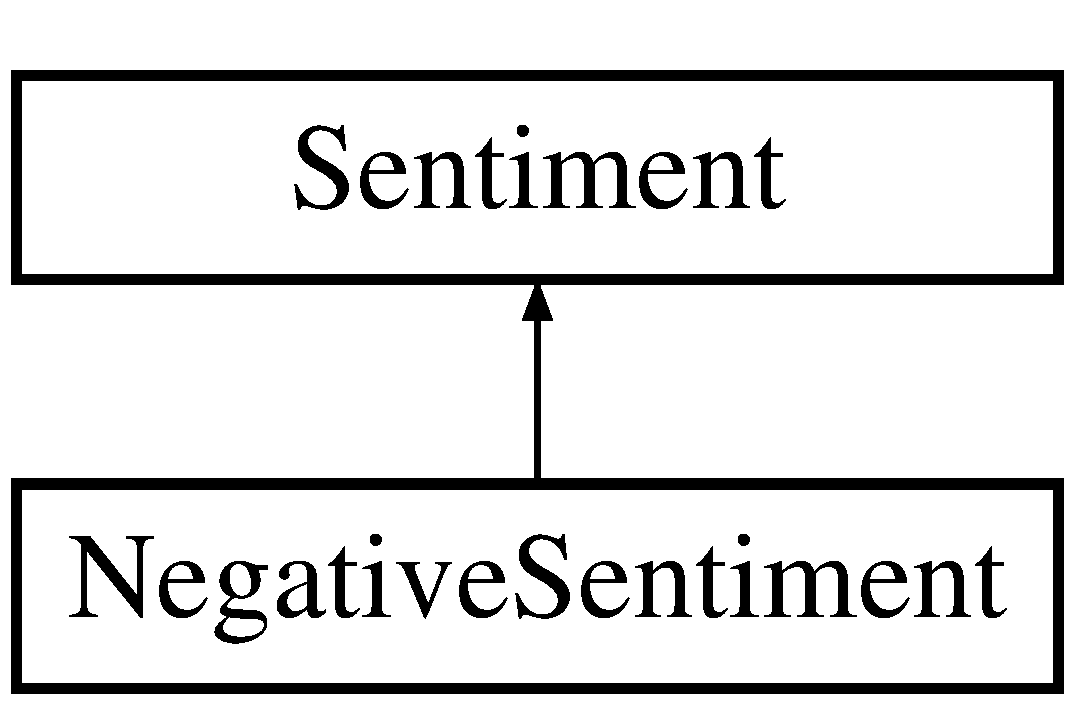
\includegraphics[height=2.000000cm]{classNegativeSentiment}
\end{center}
\end{figure}
\subsection*{Public Member Functions}
\begin{DoxyCompactItemize}
\item 
std\-::string \hyperlink{classNegativeSentiment_ae6f3705da961d94f33f93e161b1e506f}{analysis} (std\-::map$<$ std\-::string, int $>$ histogram) override
\begin{DoxyCompactList}\small\item\em analysis for \hyperlink{classNegativeSentiment}{Negative\-Sentiment} calculates the negative score for input. \end{DoxyCompactList}\item 
void \hyperlink{classNegativeSentiment_a19e8a3892275cb49ebc8b3bc2294f129}{load\-Wordlist} () override
\begin{DoxyCompactList}\small\item\em loadwordlist for the \hyperlink{classNegativeSentiment}{Negative\-Sentiment} class loads a negative wordlist. \end{DoxyCompactList}\end{DoxyCompactItemize}
\subsection*{Additional Inherited Members}


\subsection{Member Function Documentation}
\hypertarget{classNegativeSentiment_ae6f3705da961d94f33f93e161b1e506f}{\index{Negative\-Sentiment@{Negative\-Sentiment}!analysis@{analysis}}
\index{analysis@{analysis}!NegativeSentiment@{Negative\-Sentiment}}
\subsubsection[{analysis}]{\setlength{\rightskip}{0pt plus 5cm}std\-::string Negative\-Sentiment\-::analysis (
\begin{DoxyParamCaption}
\item[{std\-::map$<$ std\-::string, int $>$}]{histogram}
\end{DoxyParamCaption}
)\hspace{0.3cm}{\ttfamily [override]}, {\ttfamily [virtual]}}}\label{classNegativeSentiment_ae6f3705da961d94f33f93e161b1e506f}


analysis for \hyperlink{classNegativeSentiment}{Negative\-Sentiment} calculates the negative score for input. 

analysis takes in a histogram of input and returns a negative or positive score based on word frequency.

\begin{DoxyReturn}{Returns}
std\-::string. 
\end{DoxyReturn}


Reimplemented from \hyperlink{classSentiment_afddbb12fdb928ae171a88debef10234a}{Sentiment}.

\hypertarget{classNegativeSentiment_a19e8a3892275cb49ebc8b3bc2294f129}{\index{Negative\-Sentiment@{Negative\-Sentiment}!load\-Wordlist@{load\-Wordlist}}
\index{load\-Wordlist@{load\-Wordlist}!NegativeSentiment@{Negative\-Sentiment}}
\subsubsection[{load\-Wordlist}]{\setlength{\rightskip}{0pt plus 5cm}void Negative\-Sentiment\-::load\-Wordlist (
\begin{DoxyParamCaption}
{}
\end{DoxyParamCaption}
)\hspace{0.3cm}{\ttfamily [override]}, {\ttfamily [virtual]}}}\label{classNegativeSentiment_a19e8a3892275cb49ebc8b3bc2294f129}


loadwordlist for the \hyperlink{classNegativeSentiment}{Negative\-Sentiment} class loads a negative wordlist. 

loadwordlist for the \hyperlink{classNegativeSentiment}{Negative\-Sentiment} class preloads a dictionary of negative words. 

Reimplemented from \hyperlink{classSentiment_a5e7dabb641c08cadcab53bf92f2c3dde}{Sentiment}.



The documentation for this class was generated from the following files\-:\begin{DoxyCompactItemize}
\item 
include/Negative\-Sentiment.\-hpp\item 
app/Negative\-Sentiment.\-cpp\end{DoxyCompactItemize}

\hypertarget{classParser}{\section{Parser Class Reference}
\label{classParser}\index{Parser@{Parser}}
}
\subsection*{Public Member Functions}
\begin{DoxyCompactItemize}
\item 
\hypertarget{classParser_a12234f6cd36b61af4b50c94a179422c1}{\hyperlink{classParser_a12234f6cd36b61af4b50c94a179422c1}{Parser} ()}\label{classParser_a12234f6cd36b61af4b50c94a179422c1}

\begin{DoxyCompactList}\small\item\em Constructor \hyperlink{classParser}{Parser} Class. \end{DoxyCompactList}\item 
std\-::vector$<$ std\-::string $>$ \hyperlink{classParser_a28db3f32545756c9eec8a9bf74a8dad8}{get\-Input} ()
\begin{DoxyCompactList}\small\item\em Handles getting user input from the commandline. \end{DoxyCompactList}\item 
std\-::vector$<$ std\-::string $>$ \hyperlink{classParser_aa9014b8001ae933f1c26f692a155a029}{get\-File\-Input} (std\-::string in)
\begin{DoxyCompactList}\small\item\em Handles getting input from File exemplars or user specified files. \end{DoxyCompactList}\item 
std\-::map$<$ std\-::string, int $>$ \hyperlink{classParser_a53b6b2887c53a3fbedcd6df3cc1e69c8}{generate\-Histogram} (std\-::vector$<$ std\-::string $>$ input)
\begin{DoxyCompactList}\small\item\em generate\-Histogram takes a input vector and counts the frequency of words in that input and return a map \end{DoxyCompactList}\item 
std\-::string \hyperlink{classParser_a44db102220d866c9e6a690523e41d970}{string\-Conversion} (std\-::vector$<$ std\-::string $>$ input)
\begin{DoxyCompactList}\small\item\em string\-Coversion takes an input vector and returns string output \end{DoxyCompactList}\item 
void \hyperlink{classParser_ab605f89b56af8e8f35dcde402edac7e4}{set\-Input} (std\-::string input)
\begin{DoxyCompactList}\small\item\em set\-Input sets the input class member variable. \end{DoxyCompactList}\end{DoxyCompactItemize}


\subsection{Member Function Documentation}
\hypertarget{classParser_a53b6b2887c53a3fbedcd6df3cc1e69c8}{\index{Parser@{Parser}!generate\-Histogram@{generate\-Histogram}}
\index{generate\-Histogram@{generate\-Histogram}!Parser@{Parser}}
\subsubsection[{generate\-Histogram}]{\setlength{\rightskip}{0pt plus 5cm}std\-::map$<$ string, int $>$ Parser\-::generate\-Histogram (
\begin{DoxyParamCaption}
\item[{std\-::vector$<$ std\-::string $>$}]{input}
\end{DoxyParamCaption}
)}}\label{classParser_a53b6b2887c53a3fbedcd6df3cc1e69c8}


generate\-Histogram takes a input vector and counts the frequency of words in that input and return a map 


\begin{DoxyParams}{Parameters}
{\em input} & std\-::vector$<$std\-::string$>$ \\
\hline
\end{DoxyParams}
\begin{DoxyReturn}{Returns}
map$<$std\-::string, int$>$ 
\end{DoxyReturn}
\hypertarget{classParser_aa9014b8001ae933f1c26f692a155a029}{\index{Parser@{Parser}!get\-File\-Input@{get\-File\-Input}}
\index{get\-File\-Input@{get\-File\-Input}!Parser@{Parser}}
\subsubsection[{get\-File\-Input}]{\setlength{\rightskip}{0pt plus 5cm}std\-::vector$<$ std\-::string $>$ Parser\-::get\-File\-Input (
\begin{DoxyParamCaption}
\item[{std\-::string}]{in}
\end{DoxyParamCaption}
)}}\label{classParser_aa9014b8001ae933f1c26f692a155a029}


Handles getting input from File exemplars or user specified files. 

\begin{DoxyReturn}{Returns}
std\-::vector$<$std\-::string$>$ that contains all input from files specified by the user or file exemplars. 
\end{DoxyReturn}
\hypertarget{classParser_a28db3f32545756c9eec8a9bf74a8dad8}{\index{Parser@{Parser}!get\-Input@{get\-Input}}
\index{get\-Input@{get\-Input}!Parser@{Parser}}
\subsubsection[{get\-Input}]{\setlength{\rightskip}{0pt plus 5cm}std\-::vector$<$ std\-::string $>$ Parser\-::get\-Input (
\begin{DoxyParamCaption}
{}
\end{DoxyParamCaption}
)}}\label{classParser_a28db3f32545756c9eec8a9bf74a8dad8}


Handles getting user input from the commandline. 

Handles getting input from File exemplars or user specified files.

\begin{DoxyReturn}{Returns}
std\-::vector$<$std\-::string$>$ that contains all input from user on commandline.

std\-::vector$<$std\-::string$>$ that contains all input from files specified by the user or file exemplars. 
\end{DoxyReturn}
\hypertarget{classParser_ab605f89b56af8e8f35dcde402edac7e4}{\index{Parser@{Parser}!set\-Input@{set\-Input}}
\index{set\-Input@{set\-Input}!Parser@{Parser}}
\subsubsection[{set\-Input}]{\setlength{\rightskip}{0pt plus 5cm}void Parser\-::set\-Input (
\begin{DoxyParamCaption}
\item[{std\-::string}]{input}
\end{DoxyParamCaption}
)}}\label{classParser_ab605f89b56af8e8f35dcde402edac7e4}


set\-Input sets the input class member variable. 

set\-Input assigns a value to the \hyperlink{classParser}{Parser} class member variable input.


\begin{DoxyParams}{Parameters}
{\em input} & std\-::string \\
\hline
\end{DoxyParams}
\begin{DoxyReturn}{Returns}
string
\end{DoxyReturn}

\begin{DoxyParams}{Parameters}
{\em input} & std\-::string \\
\hline
\end{DoxyParams}
\hypertarget{classParser_a44db102220d866c9e6a690523e41d970}{\index{Parser@{Parser}!string\-Conversion@{string\-Conversion}}
\index{string\-Conversion@{string\-Conversion}!Parser@{Parser}}
\subsubsection[{string\-Conversion}]{\setlength{\rightskip}{0pt plus 5cm}std\-::string Parser\-::string\-Conversion (
\begin{DoxyParamCaption}
\item[{std\-::vector$<$ std\-::string $>$}]{input}
\end{DoxyParamCaption}
)}}\label{classParser_a44db102220d866c9e6a690523e41d970}


string\-Coversion takes an input vector and returns string output 


\begin{DoxyParams}{Parameters}
{\em input} & std\-::vector$<$std\-::string$>$ \\
\hline
\end{DoxyParams}
\begin{DoxyReturn}{Returns}
string 
\end{DoxyReturn}


The documentation for this class was generated from the following files\-:\begin{DoxyCompactItemize}
\item 
include/\hyperlink{Parser_8hpp}{Parser.\-hpp}\item 
app/\hyperlink{Parser_8cpp}{Parser.\-cpp}\end{DoxyCompactItemize}

\hypertarget{classPositiveSentiment}{\section{Positive\-Sentiment Class Reference}
\label{classPositiveSentiment}\index{Positive\-Sentiment@{Positive\-Sentiment}}
}
Inheritance diagram for Positive\-Sentiment\-:\begin{figure}[H]
\begin{center}
\leavevmode
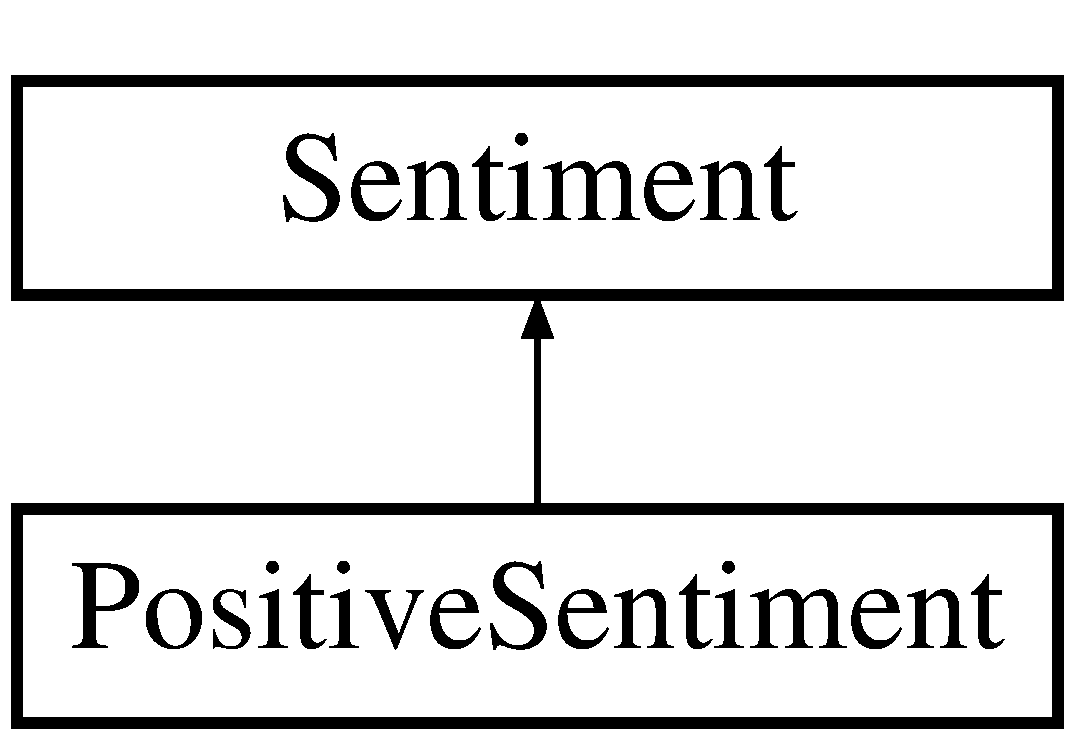
\includegraphics[height=2.000000cm]{classPositiveSentiment}
\end{center}
\end{figure}
\subsection*{Public Member Functions}
\begin{DoxyCompactItemize}
\item 
std\-::string \hyperlink{classPositiveSentiment_aeafe92c377e07ef41859a8b804563705}{analysis} (std\-::map$<$ std\-::string, int $>$ histogram) override
\begin{DoxyCompactList}\small\item\em analysis for \hyperlink{classNegativeSentiment}{Negative\-Sentiment} calculates the negative score for input. \end{DoxyCompactList}\item 
void \hyperlink{classPositiveSentiment_a980fdc3b498b3bc452255af30809b2c5}{load\-Wordlist} () override
\begin{DoxyCompactList}\small\item\em loadwordlist for the \hyperlink{classNegativeSentiment}{Negative\-Sentiment} class loads a negative wordlist. \end{DoxyCompactList}\end{DoxyCompactItemize}
\subsection*{Additional Inherited Members}


\subsection{Member Function Documentation}
\hypertarget{classPositiveSentiment_aeafe92c377e07ef41859a8b804563705}{\index{Positive\-Sentiment@{Positive\-Sentiment}!analysis@{analysis}}
\index{analysis@{analysis}!PositiveSentiment@{Positive\-Sentiment}}
\subsubsection[{analysis}]{\setlength{\rightskip}{0pt plus 5cm}std\-::string Positive\-Sentiment\-::analysis (
\begin{DoxyParamCaption}
\item[{std\-::map$<$ std\-::string, int $>$}]{histogram}
\end{DoxyParamCaption}
)\hspace{0.3cm}{\ttfamily [override]}, {\ttfamily [virtual]}}}\label{classPositiveSentiment_aeafe92c377e07ef41859a8b804563705}


analysis for \hyperlink{classNegativeSentiment}{Negative\-Sentiment} calculates the negative score for input. 

analysis takes in a histogram of input and returns a negative or positive score based on word frequency.

\begin{DoxyReturn}{Returns}
std\-::string. 
\end{DoxyReturn}


Reimplemented from \hyperlink{classSentiment_afddbb12fdb928ae171a88debef10234a}{Sentiment}.

\hypertarget{classPositiveSentiment_a980fdc3b498b3bc452255af30809b2c5}{\index{Positive\-Sentiment@{Positive\-Sentiment}!load\-Wordlist@{load\-Wordlist}}
\index{load\-Wordlist@{load\-Wordlist}!PositiveSentiment@{Positive\-Sentiment}}
\subsubsection[{load\-Wordlist}]{\setlength{\rightskip}{0pt plus 5cm}void Positive\-Sentiment\-::load\-Wordlist (
\begin{DoxyParamCaption}
{}
\end{DoxyParamCaption}
)\hspace{0.3cm}{\ttfamily [override]}, {\ttfamily [virtual]}}}\label{classPositiveSentiment_a980fdc3b498b3bc452255af30809b2c5}


loadwordlist for the \hyperlink{classNegativeSentiment}{Negative\-Sentiment} class loads a negative wordlist. 

loadwordlist for the \hyperlink{classNegativeSentiment}{Negative\-Sentiment} class preloads a dictionary of positive words. 

Reimplemented from \hyperlink{classSentiment_a5e7dabb641c08cadcab53bf92f2c3dde}{Sentiment}.



The documentation for this class was generated from the following files\-:\begin{DoxyCompactItemize}
\item 
include/Positive\-Sentiment.\-hpp\item 
app/Positive\-Sentiment.\-cpp\end{DoxyCompactItemize}

\hypertarget{classSentiment}{\section{Sentiment Class Reference}
\label{classSentiment}\index{Sentiment@{Sentiment}}
}
Inheritance diagram for Sentiment\-:\begin{figure}[H]
\begin{center}
\leavevmode
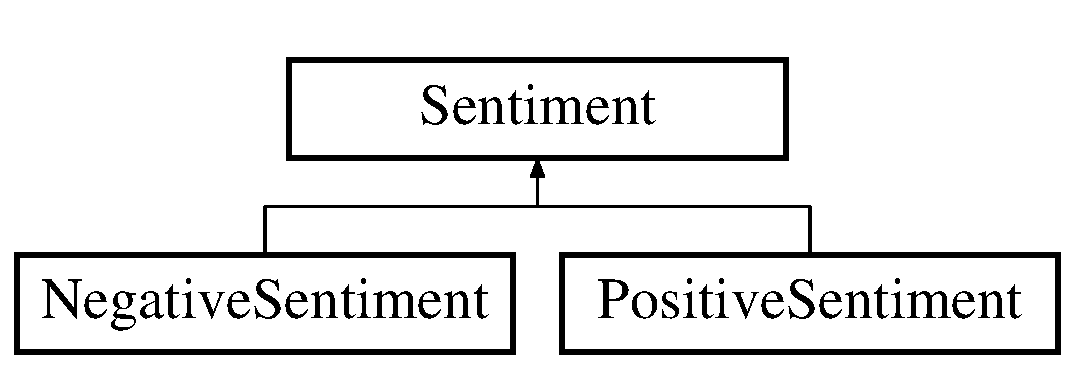
\includegraphics[height=2.000000cm]{classSentiment}
\end{center}
\end{figure}
\subsection*{Public Member Functions}
\begin{DoxyCompactItemize}
\item 
virtual std\-::string \hyperlink{classSentiment_afddbb12fdb928ae171a88debef10234a}{analysis} (std\-::map$<$ std\-::string, int $>$ histogram)
\begin{DoxyCompactList}\small\item\em analysis is a virtual function meant to be overriden by derived classes for the base classes analysis needs. \end{DoxyCompactList}\item 
\hypertarget{classSentiment_a5e7dabb641c08cadcab53bf92f2c3dde}{virtual void \hyperlink{classSentiment_a5e7dabb641c08cadcab53bf92f2c3dde}{load\-Wordlist} ()}\label{classSentiment_a5e7dabb641c08cadcab53bf92f2c3dde}

\begin{DoxyCompactList}\small\item\em loadwordlist for the \hyperlink{classSentiment}{Sentiment} class is a virtual function meant to be overriden by derived classes to define functionality for sentiment . \end{DoxyCompactList}\item 
void \hyperlink{classSentiment_aec1c59286392c42b307aade917128b45}{set\-Emotion\-Score} (int \hyperlink{classSentiment_a5a1779a5a705df433195ec737a4156ea}{emotion\-Score})
\begin{DoxyCompactList}\small\item\em set\-Emotion\-Score assigns a value to the emotionscore class member variable \end{DoxyCompactList}\item 
void \hyperlink{classSentiment_a7845d7438489c469e24ed2018b8f28cc}{set\-Wordlist} (std\-::set$<$ std\-::string $>$ \hyperlink{classSentiment_a177fabec96128aa37489b4db240535ae}{wordlist})
\begin{DoxyCompactList}\small\item\em set\-Wordlist assigns a value to the wordlist class member set \end{DoxyCompactList}\item 
\hypertarget{classSentiment_a3a88696162756d042ff19f298103fca4}{int \hyperlink{classSentiment_a3a88696162756d042ff19f298103fca4}{get\-Emotion\-Score} () const }\label{classSentiment_a3a88696162756d042ff19f298103fca4}

\begin{DoxyCompactList}\small\item\em get\-Emotion\-Score returns the value of the emotionscore class member variable \end{DoxyCompactList}\item 
\hypertarget{classSentiment_aded4e0137351e5a389a4f31be52be57b}{std\-::set$<$ std\-::string $>$ \hyperlink{classSentiment_aded4e0137351e5a389a4f31be52be57b}{get\-Wordlist} () const }\label{classSentiment_aded4e0137351e5a389a4f31be52be57b}

\begin{DoxyCompactList}\small\item\em get\-Wordlist returns the value of the wordlist class member set \end{DoxyCompactList}\end{DoxyCompactItemize}
\subsection*{Protected Types}
\begin{DoxyCompactItemize}
\item 
enum \hyperlink{classSentiment_a77da2ef7ddef68132cba46d8304a5ad1}{Emotions} \{ {\bfseries Positive} = 1, 
{\bfseries Negative} = -\/1
 \}
\begin{DoxyCompactList}\small\item\em Emotions is an Enum that keeps track of emotion score to denote a negative or positive score. \end{DoxyCompactList}\item 
enum \hyperlink{classSentiment_af2c0cb9660017b389d6d0865843742b2}{color} \{ {\bfseries Blue} = 1, 
{\bfseries Red} = -\/1
 \}
\begin{DoxyCompactList}\small\item\em color is an Enum that emotional color for Metis \end{DoxyCompactList}\end{DoxyCompactItemize}
\subsection*{Protected Attributes}
\begin{DoxyCompactItemize}
\item 
\hypertarget{classSentiment_a5a1779a5a705df433195ec737a4156ea}{int \hyperlink{classSentiment_a5a1779a5a705df433195ec737a4156ea}{emotion\-Score}}\label{classSentiment_a5a1779a5a705df433195ec737a4156ea}

\begin{DoxyCompactList}\small\item\em emotion\-Score that is used to calculate whether sentiment is negative or positive. \end{DoxyCompactList}\item 
\hypertarget{classSentiment_a177fabec96128aa37489b4db240535ae}{std\-::set$<$ std\-::string $>$ \hyperlink{classSentiment_a177fabec96128aa37489b4db240535ae}{wordlist}}\label{classSentiment_a177fabec96128aa37489b4db240535ae}

\begin{DoxyCompactList}\small\item\em wordlist is a set that holds the negative or positive wordlist. \end{DoxyCompactList}\end{DoxyCompactItemize}


\subsection{Member Function Documentation}
\hypertarget{classSentiment_afddbb12fdb928ae171a88debef10234a}{\index{Sentiment@{Sentiment}!analysis@{analysis}}
\index{analysis@{analysis}!Sentiment@{Sentiment}}
\subsubsection[{analysis}]{\setlength{\rightskip}{0pt plus 5cm}std\-::string Sentiment\-::analysis (
\begin{DoxyParamCaption}
\item[{std\-::map$<$ std\-::string, int $>$}]{histogram}
\end{DoxyParamCaption}
)\hspace{0.3cm}{\ttfamily [virtual]}}}\label{classSentiment_afddbb12fdb928ae171a88debef10234a}


analysis is a virtual function meant to be overriden by derived classes for the base classes analysis needs. 

\begin{DoxyReturn}{Returns}
std\-::string. 
\end{DoxyReturn}


Reimplemented in \hyperlink{classNegativeSentiment_ae6f3705da961d94f33f93e161b1e506f}{Negative\-Sentiment}, and \hyperlink{classPositiveSentiment_aeafe92c377e07ef41859a8b804563705}{Positive\-Sentiment}.

\hypertarget{classSentiment_aec1c59286392c42b307aade917128b45}{\index{Sentiment@{Sentiment}!set\-Emotion\-Score@{set\-Emotion\-Score}}
\index{set\-Emotion\-Score@{set\-Emotion\-Score}!Sentiment@{Sentiment}}
\subsubsection[{set\-Emotion\-Score}]{\setlength{\rightskip}{0pt plus 5cm}void Sentiment\-::set\-Emotion\-Score (
\begin{DoxyParamCaption}
\item[{int}]{emotion\-Score}
\end{DoxyParamCaption}
)}}\label{classSentiment_aec1c59286392c42b307aade917128b45}


set\-Emotion\-Score assigns a value to the emotionscore class member variable 


\begin{DoxyParams}{Parameters}
{\em int} & emotion\-Score \\
\hline
\end{DoxyParams}
\hypertarget{classSentiment_a7845d7438489c469e24ed2018b8f28cc}{\index{Sentiment@{Sentiment}!set\-Wordlist@{set\-Wordlist}}
\index{set\-Wordlist@{set\-Wordlist}!Sentiment@{Sentiment}}
\subsubsection[{set\-Wordlist}]{\setlength{\rightskip}{0pt plus 5cm}void Sentiment\-::set\-Wordlist (
\begin{DoxyParamCaption}
\item[{std\-::set$<$ std\-::string $>$}]{wordlist}
\end{DoxyParamCaption}
)}}\label{classSentiment_a7845d7438489c469e24ed2018b8f28cc}


set\-Wordlist assigns a value to the wordlist class member set 


\begin{DoxyParams}{Parameters}
{\em std\-::set$<$string$>$} & wordlist \\
\hline
\end{DoxyParams}


The documentation for this class was generated from the following files\-:\begin{DoxyCompactItemize}
\item 
include/Sentiment.\-hpp\item 
app/Sentiment.\-cpp\end{DoxyCompactItemize}

\chapter{File Documentation}
\hypertarget{Parser_8cpp}{\section{app/\-Parser.cpp File Reference}
\label{Parser_8cpp}\index{app/\-Parser.\-cpp@{app/\-Parser.\-cpp}}
}


Class that handles all input and parses it out into a format that Semantics class can use.  


{\ttfamily \#include $<$Parser.\-hpp$>$}\\*
{\ttfamily \#include $<$vector$>$}\\*
{\ttfamily \#include $<$string$>$}\\*
{\ttfamily \#include $<$iostream$>$}\\*
{\ttfamily \#include $<$algorithm$>$}\\*
{\ttfamily \#include $<$iterator$>$}\\*
{\ttfamily \#include $<$fstream$>$}\\*
{\ttfamily \#include $<$sstream$>$}\\*


\subsection{Detailed Description}
Class that handles all input and parses it out into a format that Semantics class can use. \begin{DoxyDate}{Date}
Mar 11, 2017 
\end{DoxyDate}
\begin{DoxyAuthor}{Author}
Lamar Simpson Copyright 2017 Lamar Simpson
\end{DoxyAuthor}
implementation of \hyperlink{classParser}{Parser} class. 
\hypertarget{Parser_8hpp}{\section{include/\-Parser.hpp File Reference}
\label{Parser_8hpp}\index{include/\-Parser.\-hpp@{include/\-Parser.\-hpp}}
}


\hyperlink{classParser}{Parser} Class Definition. Class designed to process user input.  


{\ttfamily \#include $<$iostream$>$}\\*
{\ttfamily \#include $<$string$>$}\\*
{\ttfamily \#include $<$map$>$}\\*
{\ttfamily \#include $<$vector$>$}\\*
\subsection*{Classes}
\begin{DoxyCompactItemize}
\item 
class \hyperlink{classParser}{Parser}
\end{DoxyCompactItemize}


\subsection{Detailed Description}
\hyperlink{classParser}{Parser} Class Definition. Class designed to process user input. \begin{DoxyCopyright}{Copyright}
G\-N\-U Public License.
\end{DoxyCopyright}
\begin{DoxyAuthor}{Author}
Lamar Simpson ( \href{https://github.com/ltsimps}{\tt https\-://github.\-com/ltsimps} ) 
\end{DoxyAuthor}
\begin{DoxyDate}{Date}
02/20/2017 
\end{DoxyDate}

%--- End generated contents ---

% Index
\newpage
\phantomsection
\addcontentsline{toc}{chapter}{Index}
\printindex

\end{document}
